% !TeX spellcheck = en_US
\section{Data and Methods}\label{sec:MethodsData}

\subsection{Data}\label{subsec:Data}

Two different datasets are used for the analysis: First, the time series of the occurrence of certain narratives described by \cite{Andre.2023} in a news corpus from the \textit{Dow Jones Newswires Machine Text Feed and Archive} database.\footnote{See  \url{https://developer.dowjones.com/site/docs/newswires_feeds/dow_jones_text_feed_and_archive/} for details.} The dataset includes content of the following areas: market-moving M\&A, exclusives, and earnings news; full-text feeds from Dow Jones sources (Newswires, The Wall Street Journal, Barron's, MarketWatch); global company news; central bank, macroeconomic, political, FX, commodities and energy news; third-party press release wires (BusinessWire, PR Newswire, Globe Newswire and others). It is important to note that the corpus includes one of the largest newspapers in the US; the Wall Street Journal.

\begin{figure}[H]
	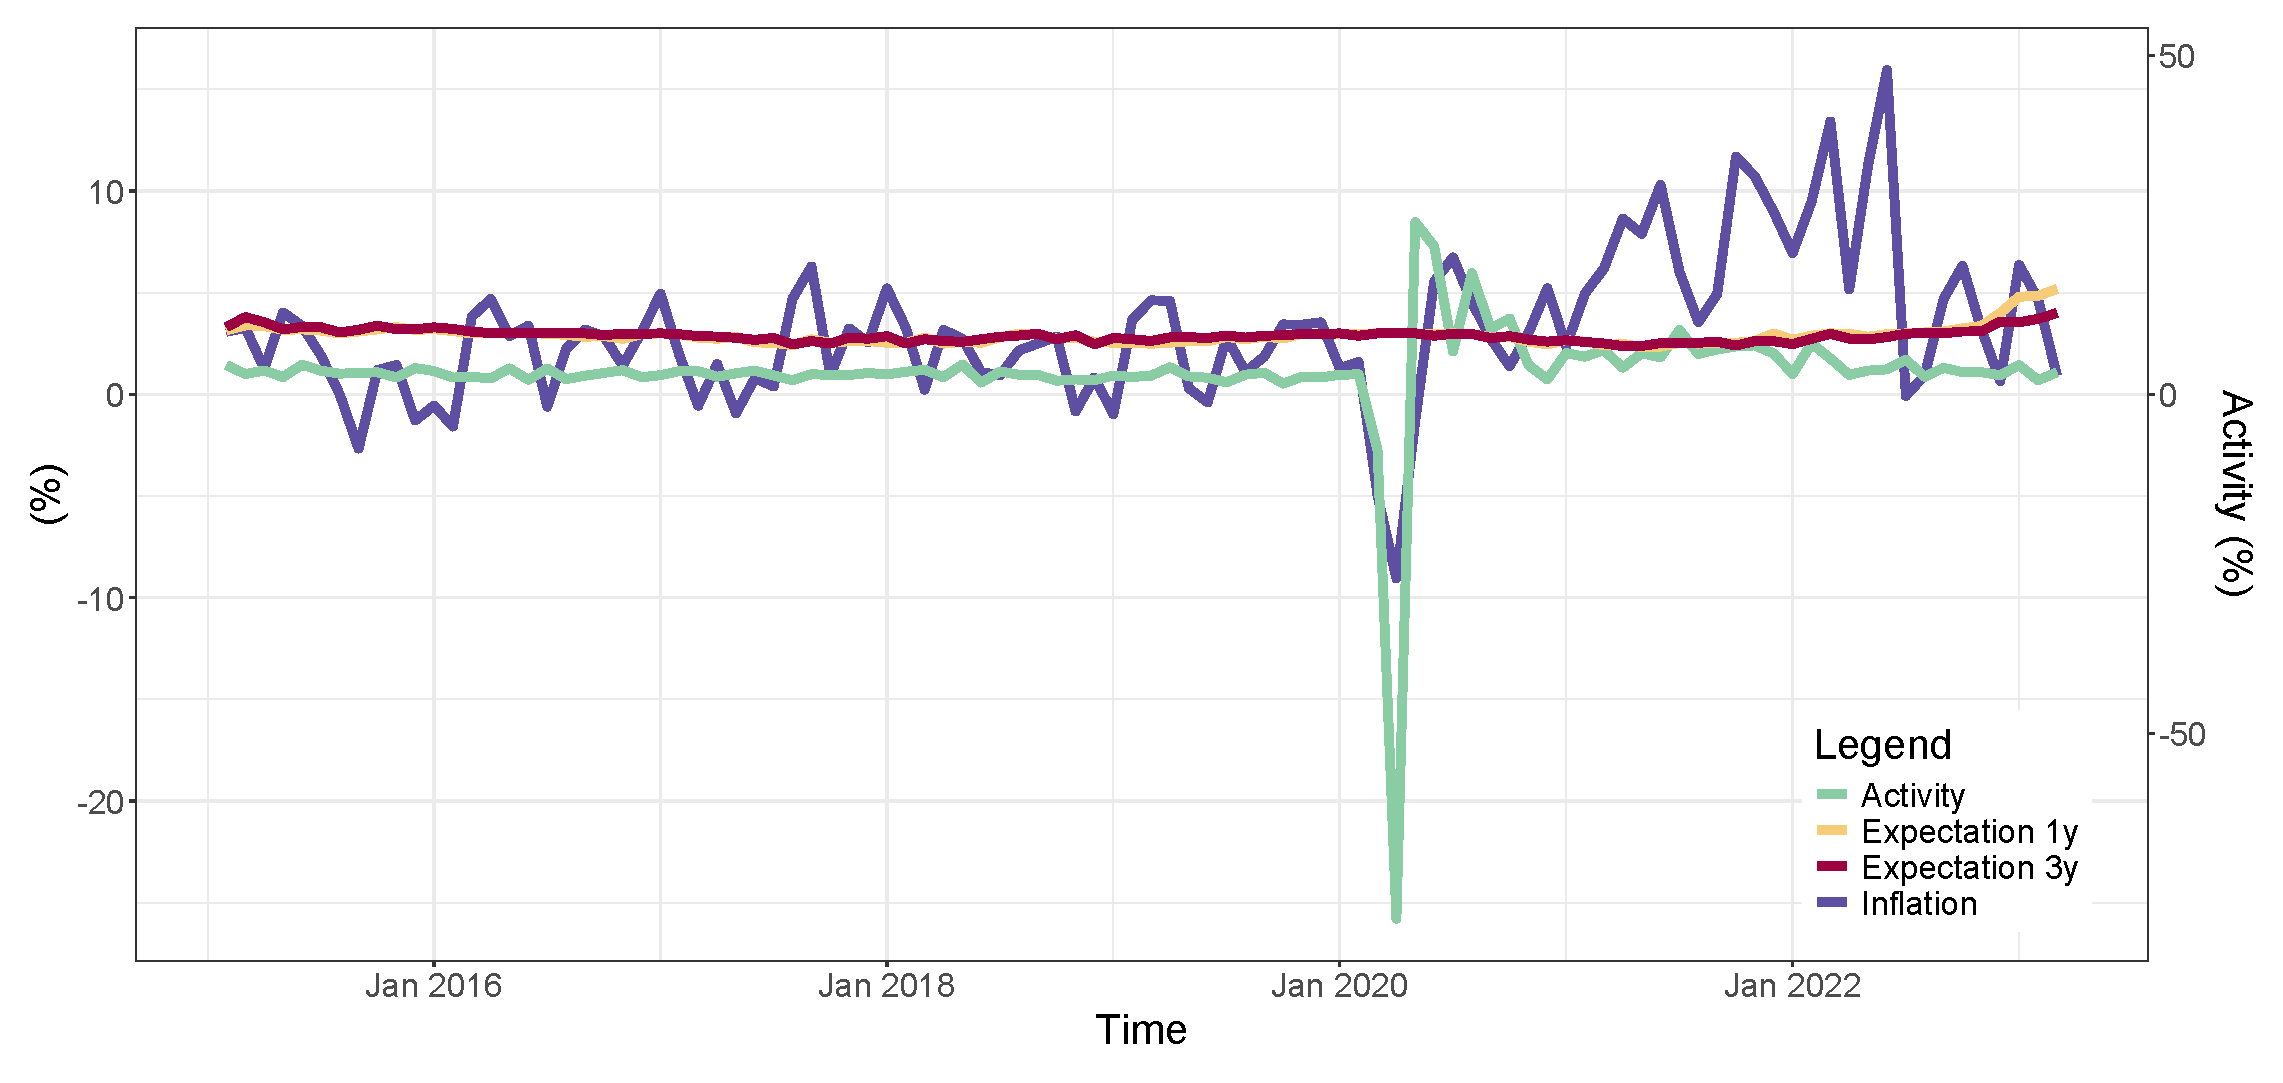
\includegraphics[width=1\linewidth]{figures/all_data.eps}
	\caption{Macroeconomic time series}
	\label{fig:alldata}
	\floatfoot{Note: `Activity' refers to the `Coincident Economic Activity Index for the United States', monthly, seasonally adjusted at annual rates. `Expectation 1y' and `Expectation 3y' refers to `New York Fed: Median 1- and 3-year ahead expected inflation rate', monthly, not seasonally adjusted. `Inflation' refers to `Consumer Price Index for All Urban Consumers: All Items in U.S. City Average', monthly, seasonally adjusted at annual rates. Source: \url{https://fred.stlouisfed.org/} and \url{https://www.newyorkfed.org/microeconomics/sce.html}}
\end{figure}

For the investigation, we use a subset of news content taken from the full corpus, filtered by keywords such as ''inflation'' for the period January 2018 to January 2023 to cover the recent inflation period. Further, the period is limited to five years due to the constrained timeliness of the survey-based measured inflation narratives in \cite{Andre.2023} and filtered by subject codes to select only relevant news sources. This amounts to a corpus of 159,440 documents. Prior to the analysis, further transformations and preprocessing steps are applied to the selected corpus, which are common when working with bag-of-words methods \citep{grimmer.2022}, e.g. lemmatization, stop words removal, constructing a document-feature matrix (see description in section \ref{subsec:DataPrep}).

Second, for the time series analysis we use a macroeconomic time series on CPI inflation (U.S. Bureau of Labor Statistics), inflation expectations (Median survey-based inflation expectations of US households one and three years ahead, New York Fed Survey) and economic activity (Coincident Economic Activity Index (CEI), Federal Reserve of Philadelphia) on a monthly basis (see figure \ref{fig:alldata}). 

CPI inflation and the economic activity index are seasonally adjusted at annual rates, while the inflation expectations are not seasonally adjusted. Moreover, as figure \ref{fig:alldata} shows, the economic activity time series contains several outliers, caused by the first Covid-19 lockdown in 2020. This may introduce a bias tp our estimations. Therefore, we treat these outliers with a dummy variable after they have been detected with the \textsf{tsoutlier()} function as implemented in \cite{forecast.2022}.

%\begin{tcolorbox}[enhanced,breakable,
%	colback=blue!5!white,colframe=blue!75!black,
%	title=To-Do]
%	
%	\begin{itemize}
%		\item Add and reference a table with all data in Appendix?
%	%	\item Document all data transformations! Year over Year on annual base??? Dlog?
%		\item Document filtering and preprocessing steps in Appendix
%	%	\item Create graphs for macroeconomic data series, same style as figure \ref{fig:inflexpect}???
%	\end{itemize}
%	
%\end{tcolorbox}

%\todo[inline]{Add and reference a table in Appendix, }

\subsection{Methods}\label{subsec:methods}

\subsubsection{Semi-supervised Keyword-assisted Topic Model (\textsf{\textbf{keyATM}})}

\cite{Eshima.2023} proposed the \textsf{keyATM} model as a semi-supervised alternative to the benchmark latent dirichlet allocation (LDA) topic model \citep{blei.2003}. They argue: ''[u]nfortunately, although topic models can \textit{explore} themes of a corpus [...], they do not necessarily \textit{measure} specific concepts of substantive interest.'' \citep[1]{Eshima.2023}. Furthermore, benchmark LDA topic models -as an unsupervised method- suffer from the post-hoc interpretability problem \citep{BoydGraber.etal.2014}.

The semi-supervised approach introduced by \cite{Eshima.2023} enables researchers to label topics by specifying keywords before fitting the model. The authors describe it as a ''semi-supervised topic model that combines a small amount of data with a large amount of unlabelled data.''\citep[2]{Eshima.2023}. The baseline \textsf{keyATM} is visualized as a plate representation in figure \ref{graph:basekeyatm} in the Online Appendix. %The proposed model is based on previous work by \cite{Jagarlamudi.etal.2012} but comes with several improvements: %First, \textsf{keyATM} can have non-keyword topics besides keyword topics. This leaves room for further exploration of the corpus. Second, the \textsf{keyATM} model can be extended with meta-information. \citep[3]{Eshima.2023}. 

Specifically, the corpus has $D$ documents and each document has $N_d$ words. $w_{di}$ stands for the $i^{th}$ word in the $d^{th}$ document. The model formulation of \textsf{keyATM} considers two types of topics: keyword topics ($\tilde{K}$) and non-keyword topics ($K$). For each keyword topic $k$ the researcher has to specify a set $L_k$ of keywords. The model is flexible enough to allow keywords to be assigned to different keyword topics simultaneously. The data generation process is modeled in such a way that at first, a latent topic variable $z_{di}$ is sampled from the topic distribution of the document $\theta_d$. If the sampled topic belongs to the non-keyword group, then the word is drawn from the corresponding word distribution of the topic ($\phi_k$). If the topic belongs to the keyword group, a Bernoulli random variable $s_{di}$ is drawn with probability $\pi_k$. This serves as an indicator variable to determine whether the word should be drawn from a set of keywords based on the probability vector $\tilde{\phi}_{k}$ or from the standard topic-word distribution $\phi$. As the estimation is based on standard Bayesian approaches, $\eta, \beta, \gamma, \tilde{\beta}$ indicate priors (see \citet[4 f.]{Eshima.2023} for a more detailed exposition).

Since the model is now based on a mixture of distributions, one with positive probabilities only for keywords on the keyword list and one with positive probabilities for all words, this implies greater prior means for the frequency of the predefined keywords than for the non-keywords in a given topic. As a result, the method is encouraged to give greater importance to keywords \textit{prior} to estimation, but to learn the exact degree of importance from the data. Thus, researchers introduce \textit{a priori} qualitative information into the estimation process of the topic model. 

For this paper we make use of specific variant of the \textsf{keyATM}, namely the \textsf{dynamic keyATM} \citep[22 ff.]{Eshima.2020}. Figure \ref{graph:dynamickeyatm} in the Online Appendix provides a plate representation of the model. As shown in the plate representation, the baseline \textsf{keyATM} is now extended by a hidden Markov model (HMM) with $R$ states where $h_{t[d]}$ denotes the latent state of document $d$ for time $t$. The transition probability matrix of the HMM is sparse, allowing only a one-step forward transition (to simplify the estimation). The \textsf{dynamic keyATM} allows the topic proportion $\theta_d$ to evolve over time by letting $\alpha$ vary across the different latent states. The authors argue that ''(m)odeling $\alpha$ instead of $\theta_d$ makes (the model) less sensitive to short-term temporal variation''. 

For the selection of the pre-specified keywords, we follow the approach of \cite{Eshima.2023} and guide our selection of keywords by the definition and example quotes by the survey study of \cite{Andre.2023}. Moreover, we take into account their results from a penalized logistic regression, which predicts whether or not a DAG factor was manually assigned to a response based on the text data. Finally, we conducted word embeddings of these keywords to optimize our selection. Accordingly, we applied an unsupervised learning algorithm for obtaining vector representations for words called GloVe by using the R Package \textsf{text2vec} \citep{text2vec.2022}. In table \ref{table:narratives}, all prior-selected keywords are listed, additionally with explanations coming from \cite{Andre.2023}. In contrast to their definitions, we use less restrictive definitions due to methodological limitations of the bag-of-words approach, which prevent us from further narrowing them down. Therefore, we treat government mismanagement as ''politics", and the price-gouging narrative as ''profits''. The pent-up demand narrative is excluded due to methodological challenges in distinguishing it from the demand (residual) narrative. Additionally, we do not consider the base effect and inflation expectations narratives, as they do not appear in the households' sample in the original study.

\subsubsection{Latent Semantic Scaling}

Our semi-supervised topic model approach allows us to quantify the prevalence of stories about the potential causes of inflation. To measure a narrative, it is important to identify the direction of its argument, e.g., whether monetary policy is causing rising or falling inflation. Both narratives may exist. Thus, it is essential to distinguish between arguments attributing the different factors to either rising or falling inflation rates. In a way, we follow the idea of ''tone-adjusted time series'' by \citep{Larsen.2019}. To ensure a distinction, simple n-gram prefiltering could be applied, utilizing n-grams such as "rising inflation" or "rising prices". This, however, would only ensure that rising inflation rates are discussed at least once in each document. A more nuanced and accurate measurement of the argument is needed. Therefore, we apply the recently proposed semi-supervised document scaling technique ''Latent Semantic Scaling'' (\textsf{LSS},  \cite{Watanabe.2021}) which is based on a word embedding approach. This allows us to develop a content-related polarity dictionary to indicate if a document is mainly about falling or rising inflation rates. 

\begin{table}[H]
	\centering
	%\scriptsize
	\begin{tabular}{l|l|l}
		\toprule
		Classification 	& ''Positive'' (= increasing) 		& ''Negative'' (= decreasing)\\
		\midrule
						& accelerate 	& decline  \\
						& acceleration  & decrease \\
						& elevate 		& deflation \\
						& high			& fall \\
						& increase		& low \\
						& persist		& lower\\
						& persistent	& reduce\\
						& pressure		& persistent\\
						& rise			& reduction\\
						& surge			& weak\\
		\bottomrule
	\end{tabular}
	\caption{Seed words for LSS initialization}\label{table:seed_words}
\end{table}


\begin{table}
	\caption{Narratives, explanations, and keywords}\label{table:narratives}
	\smallbreak
	\begin{scriptsize}
		\begin{tabular}[htp]{p{3.5cm}|p{5cm}|p{5cm}}		
			\textbf{Category}        & \textbf{Explanation}                                                                                                                                                                            & \textbf{Keywords}                                                                                                                           \\ \toprule 
			\textbf{Demand}          &                                                                                                                                                                                                 &                                                                                                                                             \\ \hline \\[0.02cm]
			Government Spending      & Increases in government spending (e.g., stimulus payments)                                                                                                                                               & infrastructure, agreement, biden, spending, deficit, bipartisan, package                                                                      \\ \\[0.02cm]
			Monetary Policy          & Loose monetary policy by the Federal Reserve                                                                                                                                                   & fed, quantitative, easing, loose, monetary, interest                                                                                        \\ \\[0.02cm]
			Pent-up Demand           & Reopening of the economy and the associated higher incomes, new spending opportunities, and optimism about the future & demand, surge, activity, recover, pandemic \\ \\[0.02cm]
			Demand Shift             & Shift of demand across sectors   (particularly increases in durables). 
			& change, consumer, good, durable, trend, service, shift, vehicle,                                                                                 \\ 
			&                                                                                                                                                                                                 &                                                                                                                                             \\
			\textbf{Supply}          &                                                                                                                                                                                                 &                                                                                                                                             \\ \midrule \\[0.02cm]
			Supply chain issues      & Disruption of global supply chains                                                                                                                                                             & supply, supplier, chain, producer, bottleneck                                                      \\ \\[0.02cm]
			Labor shortage           & Shortage of workers, e.g., due   to some workers dropping out of the labor force, and higher wage costs  & worker, employment, labor, wage, workforce, labour, job, strike, union, hire            \\ \\[0.02cm]
			Energy crisis            &  The global energy crisis,   leading to shortages of, e.g., oil and natural gas and higher energy prices 
			& crude, gas, gasoline, oil, fuel                                                                                                             \\ 
			&                                                                                                                                                                                                 &                                                                                                                                             \\
			\textbf{Miscellaneous}   &                                                                                                                                                                                                 &                                                                                                                                             \\ \hline \\[0.02cm]
			Pandemic                 & The COVID-19 pandemic, the   global pandemic recession, lockdowns, and other policy measures                                                    & pandemic, covid-19, virus, coronavirus, infection, outbreak, case                           \\ \\[0.07cm]
			Politics & Policy failure, mismanagement by   policymakers, policymakers are blamed                                                            & part, republican, trump, congress, senate, president, biden, democrats, government\\ \\[0.02cm]
			Russia-Ukraine war       & The Russian invasion of Ukraine,   the international economic, political, and military response                                               & russia, war, ukraine, invasion, moscow, putin, military                           \\ \\[0.02cm]
			Government debt          & High level of government   debt                                                                                                                                                                & debt, public, national, federal, deficit, borrowing, government, balance                                                                   \\ \\[0.02cm]
			Tax increases            & Tax increases, such as VAT   hikes                                                                                                                                                             & tax, raise, reform, legislation, overhaul, reduction\\ \\[0.02cm]
			Profits            & Greedy companies exploiting opportunities to increase profits, companies trying to make up for the money they lost during the pandemic & margin, corporate, profitability, profit, growth      \\ \\[0.02cm] \bottomrule                                                                  
		\end{tabular}
	\end{scriptsize}
\end{table}



\normalsize

Sentiment or polarity analyses are traditionally conducted by means of a dictionary approach \citep[180]{grimmer.2022}. Consequently, the major challenge is to select a domain specific dictionary or construct an own dictionary. To our knowledge, the former does not exist for the context of inflation, while the latter would be extremely time consuming. Then again, supervised machine learning methods could by applied to predict the sentiment of each document. This involves manual coding of a sufficiently large corpus, to insure reappearance of words in the training and test set, which again is time and cost intensive \citep[84]{Watanabe.2021}. In contrast, \textsf{LSS} allows us to construct our own polarity dictionary using seed and target words. Based on the proximity to a selection of seed words for each semantic dimension, polarity scores of words are computed. To estimate the semantic closeness of words, LSS recalls on singular value decomposition (SVD) of a document-feature matrix. The selected seed words are listed in table \ref{table:seed_words}. For further refinement of the polarity analysis on inflation, relevant target words are selected. Therefore, we opt for glob pattern ''infla*'' and ''price*''. Following our selection, the LSS method generates a collection of statistically significant words that occur within a window of five words around the target words. Polarity scores of words are computed as follows:

\begin{equation}
	g_f=\frac{1}{|s|}\sum_{s\in S}cos(v_s, v_f)P_s
\end{equation}


where $g_f$ are words, $s$ seed words, $p_s$ user-provided polarity of seed words, and $cos(v_s, v_f)$ the cosine similarity between the seed word vector and the word vector associated with the word f \citep[86]{Watanabe.2021}. Subsequently, the polarity scores of the documents are predicted by weighting word polarity scores by their frequency in the document: 

\begin{equation}
	y=\frac{1}{N}\sum_{f\in F}g_fh_f
\end{equation}

where $h_f$ is the frequency of words and $N$ the total number of words in the model. The documents' scores are symmetrically distributed around the mean ($\mu = 0$), and rescaled by standard deviation ($\sigma = 0$). In our case, a negative score indicates that the document is mainly about falling inflation rates, while a positive score indicates that the document is mainly about rising inflation rates. For our further analysis, we constructed narrative indices based on the document scores and the topic prevalence time series from our \textsf{keyATM} analysis. For this, we multiply the topics' proportions on the document level with the document polarity score. Finally, we aggregated our index on monthly level. 

\subsubsection{Granger Causality Tests}

In order to study the macroeconomic dynamics of our narratives, we first conducted a series of Granger causality test using our constructed narrative indices as a proxy for the narratives' virality. This allows us to study the predictive power of our narrative time series on macroeconomic variables (inflation expectations, CPI inflation, economic activity) and test their (weak) exogeneity. The Granger causality tests are constructed as multivariate tests in a vector autoregressive model (VAR) setting. The hypotheses of no Granger causality is tested by means of F test for joint significance. We follow the argument of \cite{Luetkepohl.2005}, that an $\chi^2$-distribution is often a poor approximation when working with a small sample size as ours. For our purpose we again consider five macroeconomic variables: the households' 1- and 3-year inflation expectations, the CPI inflation, the economic activity. The Granger causality statistics are used to examine whether the lagged values of one variable help to predict another one. In a more general sense we say that variable z Granger causes y if:

\begin{equation}
	\E(y_t|I_{t-1}) \neq \E(y_t|J_{t-1})
\end{equation}

\noindent Here, the vector $I_{t-1}$ contains past values of y and z, while the vector $J_{t-1}$ only contains past information on y \citep{wooldridge.2013}. Granger causality thus follows the idea that a cause cannot succeed the effect \citep[41]{Luetkepohl.2005}. 

\subsubsection{Local Projections}

To further investigate the effects of increasing narrative diffusion at the macroeconomic level, we resort to dynamic time series models and, in particular, impulse response functions (IRF). Classical tools are VARs \citep{Sims.1980}. This method, however, has some drawbacks: it is prone to mis-specification, difficult to apply to non-linear cases, and usually necessitates a relatively long lag length to ensure proper calculation \citep[161]{Jorda.2005}. The latter is of particular importance for the present study, since a rather short observation period is used. We therefore decided to estimate the dynamic response sequences on the basis of ''local projections'' (LP) method \citep{Jorda.2005}. \cite{Plagborg.2021} recently proved that under reasonable assumptions, VAR and LP estimate the same IRFs.

The basic idea of LP is to compare a conditional forecast of an event using currently available information at the time of a shock to a forecast without the shock \citep[163]{Jorda.2005}:
\begin{equation}
	IR(t,s,\bm{d}_i) = \E(\bm{y}_{t+s}|\bm{v_t} = \bm{d}_i;\bm{X}_t)-\E(\bm{y}_{t+s}|\bm{v}_t=O;\bm{X}_t), \; s = 0,1,2,...,S
\end{equation}
\noindent The operator $\E(.|.)$ denotes the best predictor of the mean square deviation, $X_t \equiv (y_{t-1},y_{t-2}...)$ and $d_i$ is a vector containing all relevant shocks. Unlike in the VAR method, the LP method estimates the impulse response using least squares regressions for each time horizon $s$ with $s=0,1,2,...S$ \citep[423]{Adaemmer.2019}:

\begin{equation}\label{eq:lp}
	\bm{y}_{t+s}=\bm{\alpha}^s+\bm{\beta}_1^{s+1}y_{t-1}+\bm{\beta}_2^{s+1}y_{t-2}+...+\bm{\beta}_p^{s+1}y_{t-p}+\bm{u}_{t+s}^s, \; s=0,1,2...,S
\end{equation}

\noindent Here, $\alpha^s$ is a vector of constants and $\beta_i^{s+1}$ are matrices with coefficients for each lag $i$ and forecast horizon $s+1$ \citep[163]{Jorda.2005}. The $\beta$ coefficients derived from the regressions are used to construct the impulse responses. Therefore, the collection of all regressions from equation \ref{eq:lp} are called \textit{Local Projections} \citep[423]{Adaemmer.2019}. The impulse responses of these local linear projections are defined as:

\begin{equation}
	\widehat{IR}(t,s,\bm{d}_i) = \hat{\bm{B}}_{1}^s\bm{d}_i, \; s=0,1,2,...,h
\end{equation}
\noindent where $\hat{\bm{B}}_1^s$ contains the coefficients of the impulse response and $\bm{d}_i$ is the vector of all relevant shocks. 

\subsubsection{Stationarity and De-trending}

The modelling of time series in VAR or ARDL models is typically based on the assumption of weak stationarity \citep[13]{Kirchgaesser.2007}. If this property is not present, there are several options: any long-run relationships that may exist can be taken into account by modelling as an error correction model, or the time series can be transformed into a stationary representation using appropriate transformations. 

Due to the short time series and the simultaneous consideration of unit root tests (see \ref{table:ers} in Online Appendix), we had to choose a trend removal approach. Simple differencing may come at costs, as such an approach may lead to information loss and spurious independence, which could result in insignificant coefficients or downward biased results \citep[201]{Kirchgaesser.2007}. However, modelling the time series at the level only makes sense if the long-term relationships are stable. We have therefore chosen another form of trend adjustment.

As \cite{hamilton.2018, phillips.2021b} have shown, applying the popular HP filter \citep{hodrick.1997} has the potential of causing an inadequate statistical trend removal leading to (worsening) spurious results, especially when the default tuning parameter is used. Several alternatives have been suggested in the literature, including the Hamilton-Filter \citep{hamilton.2018} and a boosted HP-Filter \citep{phillips.2021}. We opt for the latter, because it enables us to achieve stationarity without a loss of observation and its proved robustness with shorter sample sizes \citep{phillips.2021b}. Thus, we report our baseline estimations with trend-cycle filtered time series by means of the boosted HP-Filter. 

For robustness checks, we follow the suggestion of the literature \citep[159]{Kirchgaesser.2007} and provide level and difference estimations in the Online Appendix. Further, sufficient consideration of lags of endogenous variables should help avoid the problem of ''spurious regression'' results. To select the system's lag order, we rely on the Schwarz information criterion (SC) with a maximum of 4 lags.
 
